\documentclass[submit]{../harvardml}

\course{CS1810-S25}
\assignment{Assignment \#3}
\duedate{11:59pm EST, March 14th, 2025}

\usepackage{../common}
\usepackage[OT1]{fontenc}
\usepackage[colorlinks,citecolor=blue,urlcolor=blue]{hyperref}
\usepackage{graphicx}
\usepackage{amsmath}
\usepackage{amssymb}
\usepackage{framed}
\usepackage{color}
\usepackage{listings}
\usepackage{enumitem}
\usepackage{comment}
\usepackage{float}

%%%%%%%%%%%%%%%%%%%%%%%%%%%%%%%%%%%%%%%%%%%
%% Solution environment
\usepackage{xcolor}
\newenvironment{solution}{
    \vspace{2mm}
    \color{blue}\noindent\textbf{Solution}:
}{}
%%%%%%%%%%%%%%%%%%%%%%%%%%%%%%%%%%%%%%%%%%%

% \excludecomment{solution} % UNCOMMENT TO HIDE SOLUTIONS

% Student answer environment (used for answer templates)
\newenvironment{answer}
  {\section*{Solution}}
{}

\DeclareMathOperator*{\mean}{\mathbb{E}}

\lstset{
  language=Python,
  basicstyle=\ttfamily,
  keywordstyle=\color{blue}\bfseries,
  commentstyle=\color{red},
  stringstyle=\color{green},
  frame=single,
  showstringspaces=false,
  breaklines=true,
}

\definecolor{verbgray}{gray}{0.9}

\lstnewenvironment{csv}{%
  \lstset{backgroundcolor=\color{verbgray},
  frame=single,
  framerule=0pt,
  basicstyle=\ttfamily,
  columns=fullflexible}}{}

\begin{document}

\begin{center}
  {\Large Homework 3: Bayesian Methods and Neural Networks}\\
\end{center}

\subsection*{Introduction}

This homework is about Bayesian methods and neural networks.

\begin{enumerate}
  \item You'll explore the Bayesian paradigm and compare it with the frequentist paradigm for the Beta-Binomial conjugate pair.
  \item You'll derive the backpropagation algorithm for a single-hidden-layer neural network for the binary classification task.
  \item You'll write some code using the PyTorch library for an image classification task.
  \item You'll consider the opportunities and limitations of ML applications and learn to anticipate possible exploits of these systems.
\end{enumerate}

As always, please start early and come to office hours with questions!

\subsection*{Resources and Submission Instructions}
You may want to consider the lecture notes from Feb 18th to 27th (weeks 4 and 5).

Please type your solutions after the corresponding problems using this
\LaTeX\ template, and start each problem on a new page.

Please submit the \textbf{writeup PDF to the Gradescope assignment `HW3'}. Remember to assign pages for each question.  \textbf{You must include your plots in your writeup PDF. } The supplemental files will only be checked in special cases, e.g. honor code issues, etc.

Please submit your \textbf{\LaTeX\ file and code files to the Gradescope assignment `HW3 - Supplemental'}. \\


\newpage

%%%%%%%%%%%%%%%%%%%%%%%%%%%%%%%%%%%%%%%%%%%%%
% Problem 1
%%%%%%%%%%%%%%%%%%%%%%%%%%%%%%%%%%%%%%%%%%%%%

\begin{problem}[Connecting Bayesian and Frequentist Approaches, 40 pts]

In this question, we will gain practice with Bayesian modeling and
compare it with the frequentist paradigm.
In class, we discussed \emph{Normal-Normal conjugacy.} Now
we will turn to \emph{Beta-Binomial conjugacy.} This model can be
visualized in the following way.
You observe a fixed number \(N\) of coin flips (either
heads or tails) of which \(Y\) (a random variable) are heads. You assume that these are
drawn by flipping a coin with an unknown probability \(\theta\) of
landing heads. That is, we choose a \textbf{Binomial likelihood}
\(Y \sim \mathrm{Bin}(N, \theta)\). The PMF of this distribution is
given by

\[
  p(Y=y) = {N \choose y} \theta^{y} (1-\theta)^{N-y}.
\]

\begin{enumerate}
  \item[1.]
    \textbf{Frequentist paradigm and MLE.} The (log) likelihood is all we
    need for frequentist inference. Derive the MLE estimate for \(\theta\)
    given the observations \(Y = y\). That is, find
    \[\arg \max_{\theta} \log p(Y = y \mid \theta).\]

  \item[2.]
    \textbf{Beta-Binomial conjugacy.} Under the Bayesian paradigm, we must specify a
    prior distribution for the unknown parameter \(\theta\). We choose a \textbf{Beta prior}
    \(\theta \sim \mathrm{Beta}(\alpha, \beta)\). The PDF of this
    distribution is given by

    \[
      p(\theta) \propto \theta^{\alpha - 1} (1-\theta)^{\beta - 1}.
    \]

    When the prior and posterior belong to the same distribution family, we
    call the prior-and-likelihood pair a \textbf{conjugate pair.}

    For the rest of the problem, feel free to cite that the mean of the \(\mathrm{Beta}(\alpha, \beta)\) distribution is
    \[\mean[\theta] = \frac{\alpha}{\alpha+\beta},\]
    the mode is
    \[\arg\max_\theta p(\theta) = \frac{\alpha-1}{\alpha+\beta-2},\]
    and the variance is
    \[
      \mathrm{Var}(\theta) = \frac{\alpha \beta}{(\alpha + \beta)^2 (\alpha + \beta + 1)}.
    \]

    \begin{enumerate}
      \item
            Qualitatively speaking, what does the $\mathrm{Beta}(\alpha, \beta)$ distribution look like for different $\alpha$ and $\beta$? You can either plot this yourself or see \href{https://en.wikipedia.org/wiki/Beta_distribution}{its Wikipedia page}. What distribution does $\mathrm{Beta}(1, 1)$ correspond to?

      \item
            Show that the posterior
            \(p(\theta \mid Y=y)\) is indeed Beta and derive its parameters. This proves that a Beta prior and a Binomial likelihood form a conjugate pair; in other words, the Beta distribution is a \textbf{conjugate prior} for the Binomial distribution.

            \textbf{Hint} (for convenience in calculation): Do you need to calculate the normalizing constant?
    \end{enumerate}
\end{enumerate}
\end{problem}

\newpage

\begin{framed}
  \begin{enumerate}
    \item[3.]
      \textbf{Posterior mean and mode.} Often we wish to work with just a
      single point estimate of the posterior. Two commonly used point
      estimates are the \emph{posterior mean} and the \emph{posterior mode}
      (a.k.a. the maximum a posteriori (MAP) estimate).

      \begin{enumerate}
        \item
              Discuss the advantages and disadvantages of using posterior point
              estimates. Which of these are relevant for our Beta-Binomial conjugate pair?
        
        \item
              Using your results from part 2, write down

              \begin{enumerate}
                \item the posterior mean estimate \(\theta_{\text{post mean}} = \mean [\theta \mid Y = y]\),
                \item the posterior MAP estimate \(\theta_{\text{MAP}}=\arg \max_{\theta}p(\theta \mid Y=y)\),
                \item and the posterior variance $\mathrm{Var}(\theta \mid Y = y) = \mean[\theta^2 \mid Y = y] - (\mean[\theta \mid Y = y])^2$.
              \end{enumerate}

              \textbf{Hint}: Do you need to rederive anything? (This exercise should illustrate the power of conjugate priors!)

      \end{enumerate}

    \item[4.]
      \textbf{Prior-posterior connections.}

      \begin{enumerate}
        \item
              Explain in your own words how \(\alpha\) and \(\beta\) affect the
              MAP estimate. How would you set \(\alpha\) and \(\beta\) to reflect
              a prior belief that the coin is fair (i.e.~shows heads and tails
              with equal probability)? (Be careful that your answer does \emph{not} give high probability to an ``always heads'' coin or ``always tails'' coin!)

        \item Now let's analyze the variances of our prior and posterior distributions. Consider the case when $\alpha = \beta$. (If you'd enjoy it, consider the general case for better understanding.) Please write at most two sentences per point.
              \begin{enumerate}
                \item How does the variance of the prior relate to the variance of the posterior?
                \item How might you use the prior variance to encode a stronger or weaker prior belief?
                \item How does the posterior variance change as we observe more samples $n$?
              \end{enumerate}
      \end{enumerate}

    \item[5.]
      \textbf{Analysis and connection to frequentism.}

      \begin{enumerate}
        \item
              Write a loss function \(\ell(\theta) \in \mathbb{R}\) in terms of
              \(\theta, y, n, \alpha, \beta\) such that minimizing \(\ell\) is
              equivalent to calculating the MAP estimate,
              i.e.~\(\theta_{\text{MAP}} = \arg \min_{\theta} \ell(\theta)\). Your
              function should be a sum of:
              \begin{enumerate}
                \item a mean-squared-error term (which should loosely resemble $(y - \hat y)^2$)
                \item a
                      regularization term \(g(\theta) = - a \theta + b \theta^{2}\) for some $a, b$.
              \end{enumerate}

              Can you interpret the regularization term?

              \textbf{Hint}: Work backwards from part 1 to derive the MSE term and from the MAP in part 2 to get the regularization term. Watch out for the signs! For the interpretation, complete the square and then compare your expression with the prior mode in part 2.
        \item
              What happens to both $\theta_{\text{post mean}}$ and $\theta_{\text{MAP}}$ as \(n \to \infty\)? Compare this to the MLE estimate.
              (Remember to account for the change in \(y\).)
      \end{enumerate}

  \end{enumerate}

\end{framed}

\begin{answer}
  \begin{enumerate}
    \item[1.]
      Answer:
      \[
        \arg \max_{\theta} \log p(Y = y \mid \theta) = \frac{y}{N}
      \]
      Derivation: We first take the log of $p(Y = y | \theta)$ to get the log likelihood:
      $$\log p(Y = y | \theta) = \log\biggr({N \choose y} \theta^{y} (1-\theta)^{N-y}\biggr) = \log({N \choose y}) + y \log(\theta) + (N - y) \log ( 1- \theta)$$
      Then, to find the value of $\theta$ that maximizes this log likelihood, we diferentiate with respect to $\theta$ and set equal to $0$.
      $$\frac{\partial}{\partial \theta} \log p(Y = y | \theta) = \frac{y}{\theta} - \frac{N-y}{1-\theta} = 0$$
      Therefore, 
      $$\hat\theta = \frac{y}{N}$$
      Verifying that this is indeed a maximum, we take the second derivative of the log likelihood:
      $$\frac{\partial^2}{\partial \theta^2} \log p(Y = y | \theta) = -\frac{y}{\theta^2} - \frac{N-y}{(1-\theta)^2}$$
      Which is always negative since $y \leq N$. Therefore, since the second derivative is negative, our MLE $\hat\theta$ is a maximum.
    \item[2.]
      \begin{enumerate}
        \item
        The Beta distribution is defined over the interval $[0,1]$ and is controlled by the shape parameters $\alpha$ and $\beta$. If $\alpha, \beta > 1$, the distribution is unimodal with a peak inside $(0,1)$, while if $\alpha, \beta < 1$, it is U shaped, going to infinity at 0 and 1. When $\alpha > 1$ and $\beta < 1$, the distribution is skewed left, whereas if $\alpha < 1$ and $\beta > 1$, it is skewed right. The $\text{Beta}(1,1)$ distribution corresponds to the uniform $\text{Unif}(0,1)$ distribution.

        \item

              Parameters:
              \[
                \alpha' = \alpha + y
              \]

              \[
                \beta' = \beta + N - y
              \]

              Derivation: To find the posterior $p(\theta| Y = y)$, we use Bayes rule. For convenience of calculation, we drop the terms not dependent on $\theta$ such as the denominator $p(Y = y)$ in Bayes rule because these are simply multiplicative constants.
              $$p(\theta | Y = y) \propto p(Y = y|\theta) p(\theta)$$
              $$ \propto (\theta^{y} (1- \theta)^{N - y})  (\theta^{\alpha - 1} (1- \theta)^{\beta - 1}) = \theta^{\alpha + y - 1} (1- \theta)^{\beta + N - y - 1}$$
              Note that this is this final expression is the PDF of a Beta distribution with parameters:
              $$\text{Beta}(\alpha + y, \beta + N - y)$$
              Therefore, the posterior is
              $$p(\theta | Y =y) \sim \text{Beta}(\alpha + y, \beta + N - y)$$

      \end{enumerate}

    \item[3.]

      \begin{enumerate}
        \item
        The advantage of posterior point estimates, such as the posterior mean or mode, are that they are easier to understand since they are just values. That is, it is easier to give the mean or mode of the posterior rather than saying it is distributed as Beta with some parameters $\alpha$ and $\beta$. However, only using posterior point estimates is that they lose information on the underlying distribution. For example, just giving the mean and mode of the posterior tells us nothing about the spread of the distribution or its shape. Specifically, in the Beta Binomial case, if we have a posterior mean of $0.5$, we cannot tell if the posterior distribution is U shaped or unimodal around $0.5$, which is evidently a very important distinction. 
        \item
            We do not need to rederive anything since we found the posterior $p(\theta | Y =y)$ is distributed as $\text{Beta}(\alpha + y, \beta + n -y)$. Thus,
              \begin{align*}
                \theta_{\text{post mean}} = \mean [\theta \mid Y = y]     & = \frac{\alpha + y}{\beta + N - y}\\
                \theta_{\text{MAP}} =\arg \max_{\theta}p(\theta \mid Y=y) & = \frac{\alpha + y - 1}{\alpha + \beta + N - 2}\\
                \mathrm{Var}(\theta \mid Y = y)                           & = \frac{(\alpha + y) (\beta + N -y )}{(\alpha + \beta + N)^2(\alpha + \beta + N + 1)}
              \end{align*}
        
      \end{enumerate}

    \item[4.]

      \begin{enumerate}
        \item
        A larger $\alpha$ increases the MAP estimate while a larger $\beta$ decreases the MAP estimate. Therefore, if we wanted to encode a prior belief that the coin is fair, then we should intuitively set $\alpha = \beta$. However, we should avoid setting $\alpha = \beta = 1$ since this corresponds to a uniform distribution which would give equal probability to a fair coin, an "always heads", or an "always tails" coin. Thus, we should chose an $\alpha = \beta > 1$ since this concentrates the probability mass around $0.5$, indicating a stronger prior belief that the coin is fair. Therefore, I would set $\alpha = \beta = 2$.
        \item
              \begin{enumerate}
                \item
                The posterior variance follows the prior variance: larger prior variance means larger or larger posterior variance. However, the variance of the posterior is smaller than the variance of the prior since the $\alpha$ and $\beta$ parameters increase and the denominator of the variance from 3b grows faster than the numerator. 
                \item
                A larger prior variance encodes a weaker prior belief while a smaller prior variance encodes a stronger prior belief.
                \item
                Based on the derivation from 3b, posterior variance decreases as we observe more samples $n$. Intuitively, with more data, the more certain we are about $\theta$.
              \end{enumerate}

      \end{enumerate}

    \item[5.]

      \begin{enumerate}
        \item
              MSE term:
              \[
                M = N(\theta - \frac{y}{N} )^2
              \]

              Regularization term:
              \[
                R = -2(\alpha-1)\theta + (\alpha+\beta-2)\theta^2
              \]

              Loss function, as a function of the MSE and regularization term:
              \[
                \ell(\theta) = N\left(\frac{y}{N} - \theta\right)^2 - 2(\alpha-1)\theta + (\alpha+\beta-2)\theta^2
              \]

              MSE term derivation:
              From the hint, we want our MSE term to loosely resemble $y - \hat y)^2$. Moreover, recall from part 1 that our MLE is $\hat\theta = \frac{y}{N}$. Thus, a natural choice for the MSE term so that its minimizer is our MLE is:
              $$M = N(\theta - \frac{y}{N} )^2$$
              The term $N\left(\frac{y}{N}-\theta\right)^2$ is minimized exactly when $\theta=\frac{y}{N}$, mimicking the least-squares error $(y-\hat{y})^2$ with $\hat{y}=N\theta$. Moreover, we include the coefficient of $N$ so that the error is scaled by the number of trials.
              \\
              \\
              Regularization term derivation: Our loss function $\ell$ takes the form of MSE + a regularization term of form $g(\theta) = -a\theta + b\theta^2$. Moreover, we know that our loss should be minimized at the MAP estimate. Therefore, taking the derivative of our overall loss and setting equal to 0 should yield the MAP estimate $\theta_{MAP}$:
              $$\ell(\theta) = N\left(\theta-\frac{y}{N}\right)^2 - a\theta + b\theta^2$$
              We obtain
              $$\ell'(\theta) = 2N\left(\theta-\frac{y}{N}\right) - a + 2b\theta$$
              Setting $\ell'(\theta)=0$, we get
              $$2(N+b)\theta = 2y + a \quad \to \quad \theta = \frac{y+\frac{a}{2}}{N+b}$$
              For this to match the MAP estimate
              $$\theta_{MAP} = \frac{\alpha+y-1}{\alpha+\beta+N-2}$$
              We must have
              $$N+b = \alpha+\beta+N-2 \quad \to \quad b = \alpha+\beta-2$$
              and
              $$y+\frac{a}{2} = \alpha+y-1 \quad \to \quad a=2(\alpha-1)$$
              Therefore our regularization term is 
              $$g(\theta) = -2(\alpha - 1)\theta + (\alpha + \beta -2 )\theta^2$$
              Regularization term interpretation: The regularization term
              $$-2(\alpha-1)\theta+(\alpha+\beta-2)\theta^2$$
              When rewritten by completing the square, becomes
              $$(\alpha+\beta-2)\left(\left(\theta-\frac{\alpha-1}{\alpha+\beta-2}\right)^2 - \left(\frac{\alpha-1}{\alpha+\beta-2}\right)^2\right)$$
              Therefore, the regularization term penalizes deviations of $\theta$ from $\frac{\alpha-1}{\alpha+\beta-2}$ which means that the term will be minimized at the prior mode. This makes sense pushes $\theta$ towards the prior mode and reflects our initial belief about the most likely parameter.

        \item When $N \to \infty$, $\theta_{post \; mean}$ and $\theta_{MAP}$ both converge to $\frac{y}{N}$ since $y$ grows with $N$ so the numerator of each term will be dominated by $y$ and the denominator will be dominated by $N$. This is the exact same expression as our MLE $\hat\theta = \frac{y}{N}$. Therefore, the posterior mean and MAP both converge to our MLE as $N \to \infty$.

      \end{enumerate}

  \end{enumerate}
\end{answer}


\newpage

%%%%%%%%%%%%%%%%%%%%%%%%%%%%%%%%%%%%%%%%%%%%%
% Problem 2
%%%%%%%%%%%%%%%%%%%%%%%%%%%%%%%%%%%%%%%%%%%%%

\begin{problem}[Neural Networks, 20 pts]

In this problem, we will take a closer look at how gradients are calculated for backpropagation with a simple multi-layer perceptron (MLP). The MLP will consist of a first fully connected layer with a sigmoid activation, followed by a one-dimensional, second fully connected layer with a sigmoid activation to get a prediction for a binary classification problem. We use non-linear activation functions as the composition of linear functions is linear. Assume bias has not been merged. Let:
\begin{itemize}
  \item $\bold{W}_1$ be the weights of the first layer, $\bold{b}_1$ be the bias of the first layer.
  \item $\bold{W}_2$ be the weights of the second layer, $\bold{b}_2$ be the bias of the second layer.
\end{itemize}

The described architecture can be written mathematically as: $$\hat{y} = \sigma(\bold{W}_2 \left[\sigma \left(\bold{W}_1 \bold{x} + \bold{b}_1\right)\right] + \bold{b}_2)$$

where $\hat{y}$ is a scalar output of the net when passing in the single datapoint $\bold{x}$ (represented as a column vector), the additions are element wise additions, and the sigmoid is an element wise sigmoid.

\begin{enumerate}
  \item Let:
        \begin{itemize}
          \item $N$ be the number of datapoints we have
          \item $M$ be the dimensionality of the data
          \item $H$ be the size of the hidden dimension of the first layer. Here, hidden dimension is used to describe the dimension of the resulting value after going through the layer. Based on the problem description, the hidden dimension of the second layer should be 1.
        \end{itemize}

        Write out the dimensionality of each of the parameters, and of the intermediate variables:

        \begin{align*}
          \bold{a}_1 & = \bold{W}_1 \bold{x} + \bold{b}_1,
                     & \bold{z}_1 = \sigma(\bold{a}_1)       \\
          a_2        & = \bold{W}_2 \bold{z}_1 + \bold{b}_2,
                     & \hat{y} = z_2 = \sigma(a_2)
        \end{align*}

        and make sure they work with the mathematical operations described above. Examining shapes is one of the key ways to debug your code, and can be done using .shape after any numpy array.

  \item  We will derive the gradients for each of the parameters, which can then be used along with gradient descent to find weights that improve our model's performance. For this question, assume there is only one datapoint $\bold{x}$, and that our loss is $L = -(y \log (\hat{y}) + (1 - y) \log (1 - \hat{y}))$. For all questions, the chain rule will be useful.
        \begin{enumerate}
          \item Find $\frac{\partial L}{\partial b_2}$.
            
          \item Find $\frac{\partial L}{\partial W_2^h}$, where $W_2^h$ represents the $h$th element of $\bold{W}_2$.

          \item Find $\frac{\partial L}{\partial b_1^h}$, where $b_1^h$ represents the $h$th element of $\bold{b}_1$. (\textbf{Hint}: Note that only the $h$th element of $\bold{a}_1$ and $\bold{z}_1$ depend on $b_1^h$ - this should help you with how to use the chain rule.)

          \item Find $\frac{\partial L}{\partial W_1^{h, j}}$, where  $W_1^{h,j}$ represents the element in row $h$, column $j$ in $\bold{W}_1$.

        \end{enumerate}

\end{enumerate}

\end{problem}

\newpage

\begin{framed}
  \noindent\textbf{Problem 2} (cont.)\\
  \begin{enumerate}
    \setcounter{enumi}{2}

    \item  We now explore an example of forward-mode auto-differentiation. Consider the following
          equation:

          $$
            f(x_1, x_2) = \ln (\sin (x_1)) + x_1 \exp \{ x_2 \}
          $$

          This equation can be split up using intermediate variables $v_1, \dots, v_7$ as follows:

          \begin{align*}
            v_1         & = x_1            \\
            v_2         & = \sin (v_1)     \\
            v_3         & = \ln (v_2)      \\
            v_4         & = x_2            \\
            v_5         & = \exp \{ v_4 \} \\
            v_6         & = v_1v_5         \\
            v_7         & = v_3 + v_6      \\
            f(x_1, x_2) & = v_7
          \end{align*}

          Splitting up the equation like this is very similar to what an auto-differentiation
          library would do. From these equations we can construct a \textit{computational graph}
          where each node of the graph corresponds to an input, an intermediate variable, or
          the output.

          \begin{enumerate}
            \item Let $x_1 = \frac{\pi}{6}$ and $x_2 = 1$. Calculate the values of all the
                  intermediate variables $v_1, \dots v_7$ and $f(x_1,x_2)$.
            \item Calculate the derivative of
                  all of the intermediate variables $v_1, \dots, v_7$ and
                  $f$ with respect to $x_1$ evaluated
                  at $x_1 = \frac{\pi}{6}$ and $x_2 = 1$. Remember to write out the equations before evaluating, e.g.,
                  \[
                    \frac{\partial f(x)}{\partial x} = \frac{\partial f(x)}{\partial g(x)} \frac{\partial g(x)}{\partial x}.
                  \]
          \end{enumerate}
  \end{enumerate}
\end{framed}

\begin{answer}
  \begin{enumerate}
    \item Since $\bold{x}$ is given in the problem as a column vector of size $M \times 1$. We also know that our output is a scalar so our output $\hat y$  has dimension $1 \times 1$.  Therefore, we must have the following dimensions:
    \begin{itemize}
            \item $\bold{W}_1 : H \times M$
            \item $\bold{b}_1 : H \times 1$
            \item $\bold{W}_2 : 1 \times H$
            \item $\bold{b}_2 : 1 \times 1$
            \item $\bold{a}_1 : H \times 1$
            \item $\bold{z}_1 : H \times 1$
            \item $a_2 : 1 \times 1$
            \item $\hat{y} : 1 \times 1$
          \end{itemize}

    \item Applying chain rule, we get
        \begin{enumerate}
            \item
                  \begin{align*}
                    \frac{\partial L}{\partial b_2} = \frac{\partial L}{\partial \hat{y}} \cdot \frac{\partial \hat{y}}{\partial a_2} \cdot \frac{\partial a_2}{\partial b_2} = \left(-\frac{y}{\hat{y}} + \frac{1-y}{1-\hat{y}}\right)
                    \cdot \hat{y}(1-\hat{y}) \cdot 1 = \hat{y}-y
                  \end{align*}

            \item
                  \begin{align*}
                    \frac{\partial L}{\partial W_2^h} = \frac{\partial L}{\partial \hat{y}} \cdot \frac{\partial \hat{y}}{\partial a_2} \cdot \frac{\partial a_2}{\partial W_2^h} = \left(-\frac{y}{\hat{y}} + \frac{1-y}{1-\hat{y}}\right)
                    \cdot \hat{y}(1-\hat{y}) \cdot z_1^h = (\hat{y}-y) z_1^h.
                  \end{align*}

            \item
                  \begin{align*}
                    \frac{\partial L}{\partial b_1^h} 
                    &= \frac{\partial L}{\partial \hat{y}} \cdot \frac{\partial \hat{y}}{\partial a_2} \cdot \frac{\partial a_2}{\partial z_1^h} \cdot \frac{\partial z_1^h}{\partial a_1^h} \cdot \frac{\partial a_1^h}{\partial b_1^h} \\
                    &= \left(-\frac{y}{\hat{y}} + \frac{1-y}{1-\hat{y}}\right)
                    \cdot \hat{y}(1-\hat{y}) \cdot W_2^h \cdot \left(z_1^h(1-z_1^h)\right) \cdot 1 \\
                    &= (\hat{y}-y) W_2^h  z_1^h (1-z_1^h).
                  \end{align*}

            \item
                  \begin{align*}
                    \frac{\partial L}{\partial W_1^{h,j}} 
                    &= \frac{\partial L}{\partial \hat{y}} \cdot \frac{\partial \hat{y}}{\partial a_2} \cdot \frac{\partial a_2}{\partial z_1^h} \cdot \frac{\partial z_1^h}{\partial a_1^h} \cdot \frac{\partial a_1^h}{\partial W_1^{h,j}} \\
                    &= \left(-\frac{y}{\hat{y}} + \frac{1-y}{1-\hat{y}}\right)
                    \cdot \hat{y}(1-\hat{y}) \cdot W_2^h \cdot \left(z_1^h(1-z_1^h)\right) \cdot x^j \\
                    &= (\hat{y}-y) W_2^h z_1^h (1-z_1^h) x^j
                  \end{align*}
          \end{enumerate}

    \item

          \begin{enumerate}
            \item Plugging in $x_1 = \frac{\pi}{6}$ and $x_2 = 1$ to the given variables, we get
                  \begin{align*}
                    v_1        & = \frac{\pi}{6}\\
                    v_2        & = \frac{1}{2}\\
                    v_3        & = -\ln 2\\
                    v_4        & = 1\\
                    v_5        & = e\\
                    v_6        & = \frac{\pi e}{6}\\
                    v_7        & = -\ln2 + \frac{\pi e}{6}\\
                    f(x_1,x_2) & = -\ln 2 + \frac{\pi e}{6}\\
                  \end{align*}

            \item Evaluated at $x_1 = \frac{\pi}{6}$ and $x_2 = 1$ and applying chain rule when necessary, we get
                  \begin{align*}
                    \frac{\partial v_1}{\partial x_1} & = 1\\
                    \frac{\partial v_2}{\partial x_1} & = \frac{\partial v_2}{\partial v_1} \frac{\partial v_1}{\partial x_1} = \cos(v_1) \cdot 1 = \cos (\frac{\pi}{6}) = \frac{\sqrt{3}}{2}\\
                    \frac{\partial v_3}{\partial x_1} & = \frac{\partial v_3}{\partial v_2} \frac{\partial v_2}{\partial x_1} = \frac{1}{v_2}\cdot \frac{\sqrt{3}}{2} = 2\cdot \frac{\sqrt{3}}{2} = \sqrt{3}\\
                    \frac{\partial v_4}{\partial x_1} & = \frac{\partial v_4}{\partial x_2} \frac{\partial x_2}{\partial x_1} = 1 \cdot 0 = 0\\
                    \frac{\partial v_5}{\partial x_1} & = \frac{\partial v_5}{\partial v_4} \frac{\partial v_4}{\partial x_1} = e^{v_4} \cdot 0 = 0\\
                    \frac{\partial v_6}{\partial x_1} & = v_1\frac{\partial v_5}{\partial x_1} + v_5\frac{\partial v_1}{\partial x_1} = \frac{\pi}{6} \cdot 0 + e \cdot 1 = e\\
                    \frac{\partial v_7}{\partial x_1} & = \frac{\partial v_3}{\partial x_1} + \frac{\partial v_6}{\partial x_1} = \sqrt{3} + e\\
                    \frac{\partial f}{\partial x_1}   & =\frac{\partial f(x_1,x_2)}{\partial v_7} \frac{\partial v_7}{\partial x_1} = 1 \cdot (\sqrt{3} + e) = \sqrt{3} + e
                  \end{align*}
          \end{enumerate}

  \end{enumerate}
\end{answer}


\newpage

%%%%%%%%%%%%%%%%%%%%%%%%%%%%%%%%%%%%%%%%%%%%%
% Problem 3
%%%%%%%%%%%%%%%%%%%%%%%%%%%%%%%%%%%%%%%%%%%%%

\begin{problem}[Modern Deep Learning Tools: PyTorch, 40 pts]

In this problem, you will learn how to use PyTorch. This machine learning library is massively popular and used heavily throughout industry and research.


\begin{enumerate}
  \item In \verb|homework3.ipynb| you will implement an MLP for image classification from scratch. Paste your code solutions below and include a final graph of your training progress. Also, submit your completed \verb|homework3.ipynb| file.
  \item Discuss what trends you see with your plot (train/test loss and train/test accuracy).
  \item \textbf{Out of Distribution (OOD) Analysis}: Now, let's evaluate the usefulness of the predictive uncertainties of our model for test data that are dissimilar to our training data. These test data points are called out of distribution (OOD) points. Report both the in and out distribution test accuracies of your model. In a couple of sentences, discuss what you notice about these accuracies.

  \item Now let us consider the implications of what we have seen.  First, just as in Homework 2, we want the predictive uncertainties from our models to help us distinguish in-distribution test data (test data that are similar to data on which we trained our model) and OOD test data.  Look at some examples in which the model expresses uncertainty about an in-distribution output and in which the model expresses uncertainty about an out-of-distribution output.  Characterize what you see.  In what ways are the uncertainties of the model useful, and in what ways are they not?  Do you think training multiple models and boostrapping, like you did in Homework 2, would help?  (You do not have to code anything, just discuss.)

  \item Suppose the postal service was going to use your model to help automatically sort mail by zipcodes (a real use of AI systems).  They want to make sure that their system is safe against adversarial attacks.  Let us suppose that the model is relatively safe against software attacks, that is, appropriate security is in place such that the adversary cannot simply change the weights of a deployed model without someone noticing (in practice, this would be an important element).  Three scenarios, however, are of concern to them:
        \begin{enumerate}
          \item Hardware attack: Suppose the adversary has access to the
                scanner used to take pictures of the envelopes.  How might
                they be able to change the outputs of the model to their
                desired ones?  What safeguards might be possible, and what
                are their benefits and limitations/drawbacks?
          \item Input attack: Suppose the adversary has access to the
                envelopes prior to scanning.  How might they be able to
                change the outputs of the model to their desired ones?
                What safeguards might be possible, and what are their
                benefits and limitations/drawbacks?
          \item Social Engineering attack: Suppose that the adversary
                has access to the teams that will be maintaining and
                retraining the model.  How might they be able to change the
                outputs of the model to their desired ones?  What safeguards
                might be possible, and what are their benefits and
                limitations/drawbacks?
        \end{enumerate}
        \textbf{In no more than 10 lines}, consider possible safeguards that might be implemented to the software, system integration, and work environment overall?  You may find
        it useful to explore how you can manipulate your model by
        changing inputs, etc. but no coding is required for this
        question.

\end{enumerate}

{\bfseries You will recieve no points for code not included below.}

{\bfseries You will recieve no points for code using built-in APIs from the \verb|torch.nn| library.}

\end{problem}


\begin{answer}

  \begin{enumerate}
    \item[1.]

      Plot: 
      \begin{figure}[H]
          \centering
          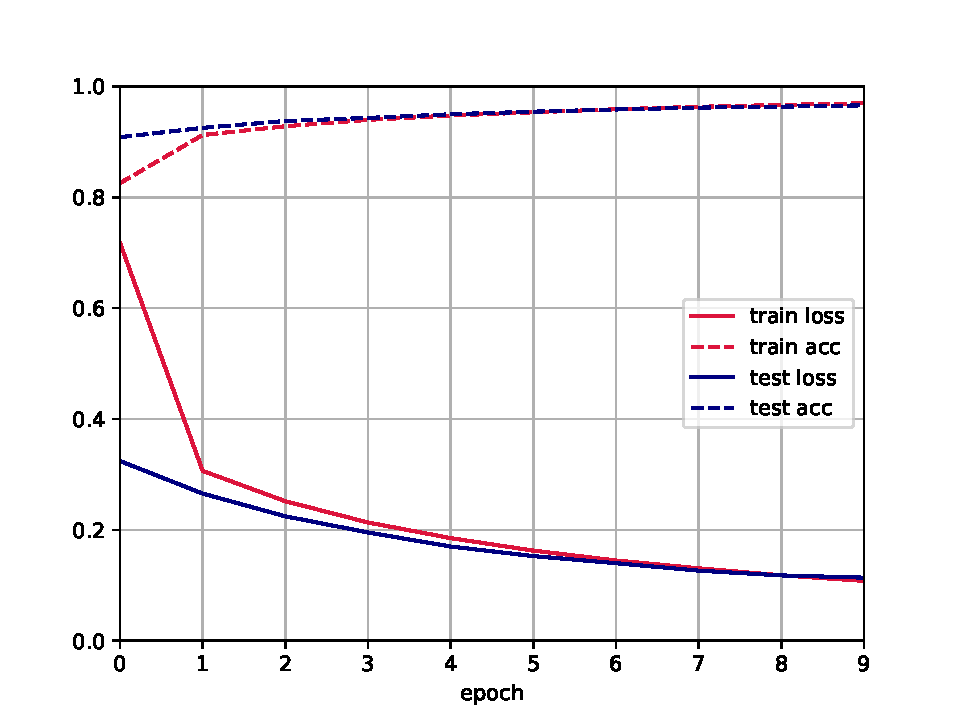
\includegraphics[width=0.8\linewidth]{hw3/final_plot.pdf}
      \end{figure}
      \begin{figure}[H]
          \centering
          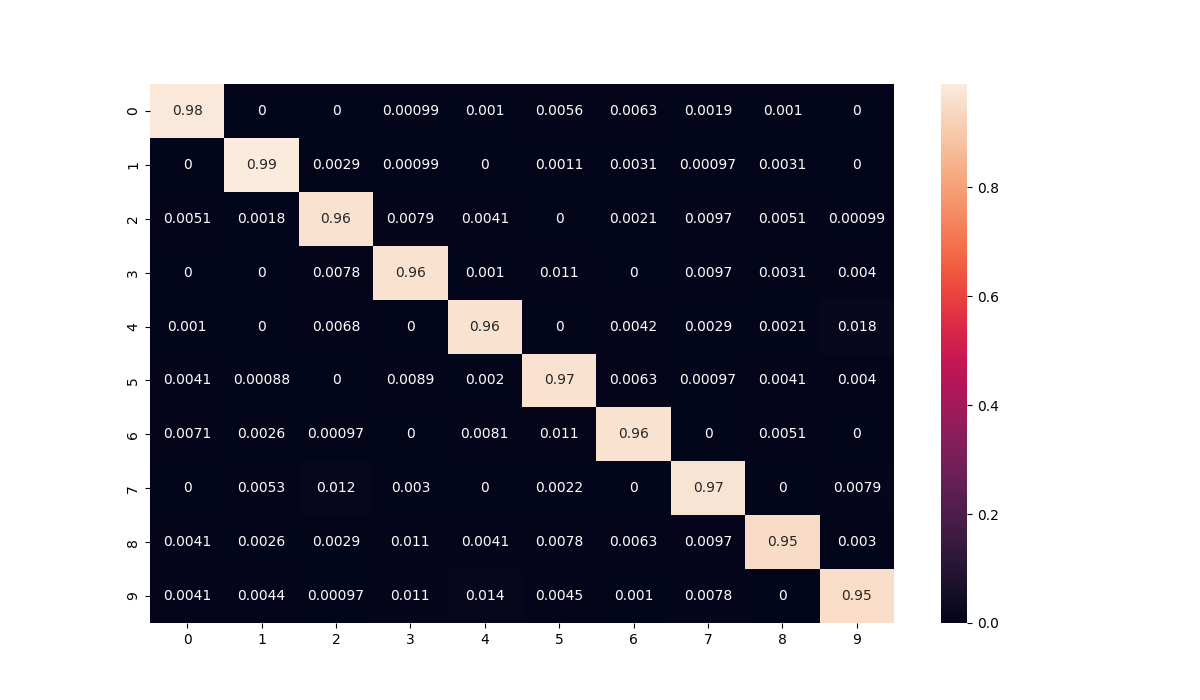
\includegraphics[width=0.9\linewidth]{hw3/confusion_matrix.png}
      \end{figure}

      Code:

      \begin{lstlisting}[language=Python]
# Flattened image size 
n_inputs = 28 * 28

# Given J = 256
n_hiddens = 256

# 10 digits possible
n_outputs = 10

W1 = torch.nn.Parameter(torch.randn(size = (n_inputs, n_hiddens)) * 0.01)
b1 = torch.nn.Parameter(torch.zeros(size = (1,n_hiddens)))
W2 = torch.nn.Parameter(torch.randn(size = (n_hiddens, n_outputs)) * 0.01)
b2 = torch.nn.Parameter(torch.zeros(size = (1,n_outputs)))

params = [W1, b1, W2, b2]

def relu(x):
  return torch.clamp(x, min = 0)

def softmax(X):
  # Divide exponentiated X by row wise sum
  return torch.exp(X) / torch.sum(torch.exp(X), dim=1, keepdim=True)


def net(X):
  # Flatten the input into 2D array of batch size x flattened image size (start flattening at dim 1)
  flattened_X = torch.flatten(X, start_dim=1)  

  # Compute hidden layer activation
  H = relu(flattened_X @ W1 + b1)

  # Compute output layer with softmax
  O = softmax(H @ W2 + b2)
  
  return O



def cross_entropy(y_hat, y):
  batch_size = y_hat.shape[0]
  return -torch.log(y_hat[torch.arange(batch_size), y])



def sgd(params, lr=0.1):
  with torch.no_grad():
    for p in params:
      p -= lr * p.grad 
      p.grad.zero_() 



def train(net, params, train_iter, loss_func=cross_entropy, updater=sgd):
  for epoch in range(10):
    for X, y in train_iter:
      # Forward pass
      y_hat = net(X)

      # Compute loss
      loss = loss_func(y_hat, y).mean()

      # Backward pass
      loss.backward()

      # Update params
      updater(params)

\end{lstlisting}

    \item[2.] As the epochs progress, the test and training losses decrease dramatically while the test and training accuracies increase. While the training accuracy starts off slightly below the testing accuracy, the accuracies begin to match at epoch 4 and plateau around 0.95. On the other hand, the training loss is initially much larger than testing loss but the two losses begin to match each other at epoch 7. The initial difference is likely due to the high training losses incurred while beginning to learn the optimal parameters. Notably, since the training and testing accuracy both converge to 0.95, this suggests that the model will generalize well to in distribution data.

    \item[3.]

      Test Accuracy (In Distribution): 0.9959

      Test Accuracy (Out of Distribution): 0.0

      Discussion: Our model has near perfect accuracy (99.5\% test accuracy) on in distribution data yet fails completely (0\% test accuracy) on out of distribution data. This indicates that our model is failing to generalize its predictions beyond data that is similar to what it has seen before. Specifically, since we only train our model on digits 1 and 6 in the MNIST dataset, then when we present an input labeled 3 the model has no idea how to classify this point as the only digits it has ever seen before has been 1 and 6. 

    \item[4.] On some examples, the model outputs a nearly flat probability distribution over the classes which indicates uncertainty. For such in-distribution examples, this is usually when the number itself is ambiguous such as when the number is smudged or poorly written. Thus, regardless of the model, these in-distribution examples are naturally "hard" examples to correctly classify. On the other hand, for out of distribution examples, the model is extremely uncertain even if the number is very clear to a human reader. In this case, we attribute the uncertainty in the model based on a systemic error in the model: since the model has never seen the digit $3$ during its training, it has no clue how to classify this new data point.
    \\
    \\
    The uncertainties of the model can be useful in that they reflect additional information about the data itself-- in the in distribution case, the model implicitly encodes information about how ambiguous the digit is drawn which can be used to flag potentially unusable data. However, model uncertainty can also be very tricky to deal with. Consider the case in part 5 of this question. If the model is presented with an out of distribution digit on a post card and incorrectly classifies it (ie. choosing the one class that has marginally higher probability than the rest), then the mailing system could break down as mail is sent to the wrong place consistently.
    \\
    \\
    I think training multiple models and bootstrapping could help with this issue. This approach could provide more reliable uncertainty estimates by averaging over multiple models rather than relying on a single model’s confidence. If each model is trained on slightly different subsets of the data, their collective predictions could help distinguish between genuine uncertainty (ie. ambiguous in-distribution examples) and true out-of-distribution cases. Additionally, bootstrapping could help reduce overconfidence by smoothing out individual model biases, potentially leading to a more calibrated confidence measure. However, this approach is computationally expensive and might still struggle if the out-of-distribution data is entirely disjoint from the training distribution.

    \item[5.] 

      \begin{enumerate}
        \item  If an adversary has access to the scanner used to capture images of envelopes, they could manipulate physical conditions to distort the model’s input (changing resolution, changing lighting, etc). This could cause misclassification, leading to mail being incorrectly routed. A possible safeguard is to use multiple redundant scanners and manually validate the outputs with confidence under a certain threshold. However, these safeguards might not fully prevent a determined attacker and would introduce costs through additional computational overhead.
        \item If an adversary has access to the envelopes before scanning, they could modify the actual zipcodes themselves before the model classifies them. A possible safeguard against this would be limiting access to envelopes through stricter and more secure protocols, although this might not be possible if much of the mailing operations cannot be automated.
        \item If an adversary can influence the teams maintaining and retraining the model, they could introduce biased training data, poisoning the system to systematically misclassify certain digits in zipcodes. A safeguard here would be to implement model update logs, auditing, and deeper background checks on employees, although this would cost additional resources.
      \end{enumerate}


  \end{enumerate}

\end{answer}


%%%%%%%%%%%%%%%%%%%%%%%%%%%%%%%%%%%%%%%%%%%%%
% Name and Calibration
%%%%%%%%%%%%%%%%%%%%%%%%%%%%%%%%%%%%%%%%%%%%%
\newpage
\subsection*{Name}
Jaray Liu
\subsection*{Collaborators and Resources}
Whom did you work with, and did you use any resources beyond cs181-textbook and your notes?


\end{document}
